\subsection{General description}

The GeoPAT consists of twelve modules.
Five modules are designed for extracting pattern signatures from an original data grid, four modules for actual geoprocessing of the patterns and three utility modules.

The role of signature extraction modules (gpat\_gridhis, gpat\_gridts, gpat\_pointshis, gpat\_pointsts, gpat\_polygon) is to calculate pattern signatures for scenes defined:

\begin{itemize}
  \item gpat\_gridhis - by a neighborhood of each cell in a grid (spatial pattern)
  \item gpat\_gridts - by a neighborhood of each cell in a grid (spatiotemporal pattern)
  \item gpat\_pointshis - in the neighborhoods of selected points (spatial pattern)
  \item gpat\_pointsts - in the neighborhoods of selected points (spatiotemporal pattern)
  \item gpat\_polygon - over irregular polygons
\end{itemize}

The role of geoprocessing modules (gpat\_search, gpat\_compare, gpat\_segment, gpat\_distmtx) is to perform:

\begin{itemize}
  \item gpat\_search - searching
  \item gpat\_compare - comparision
  \item gpat\_segment - segmentation (based on pattern data generated by the signature extraction modules)
  \item gpat\_distmtx - clustering
\end{itemize}

The role of utility modules (gpat\_grd2txt, gpat\_globnorm, gpat\_segquality) is to:

\begin{itemize}
  \item gpat\_grd2txt - 
  \item gpat\_globnorm - 
  \item gpat\_segquality - calculate the quality metrics (inhomogeneity and isolation) of a segmentation
\end{itemize}

\begin{figure}[H]
%	\centering
	\makebox[\textwidth][c]{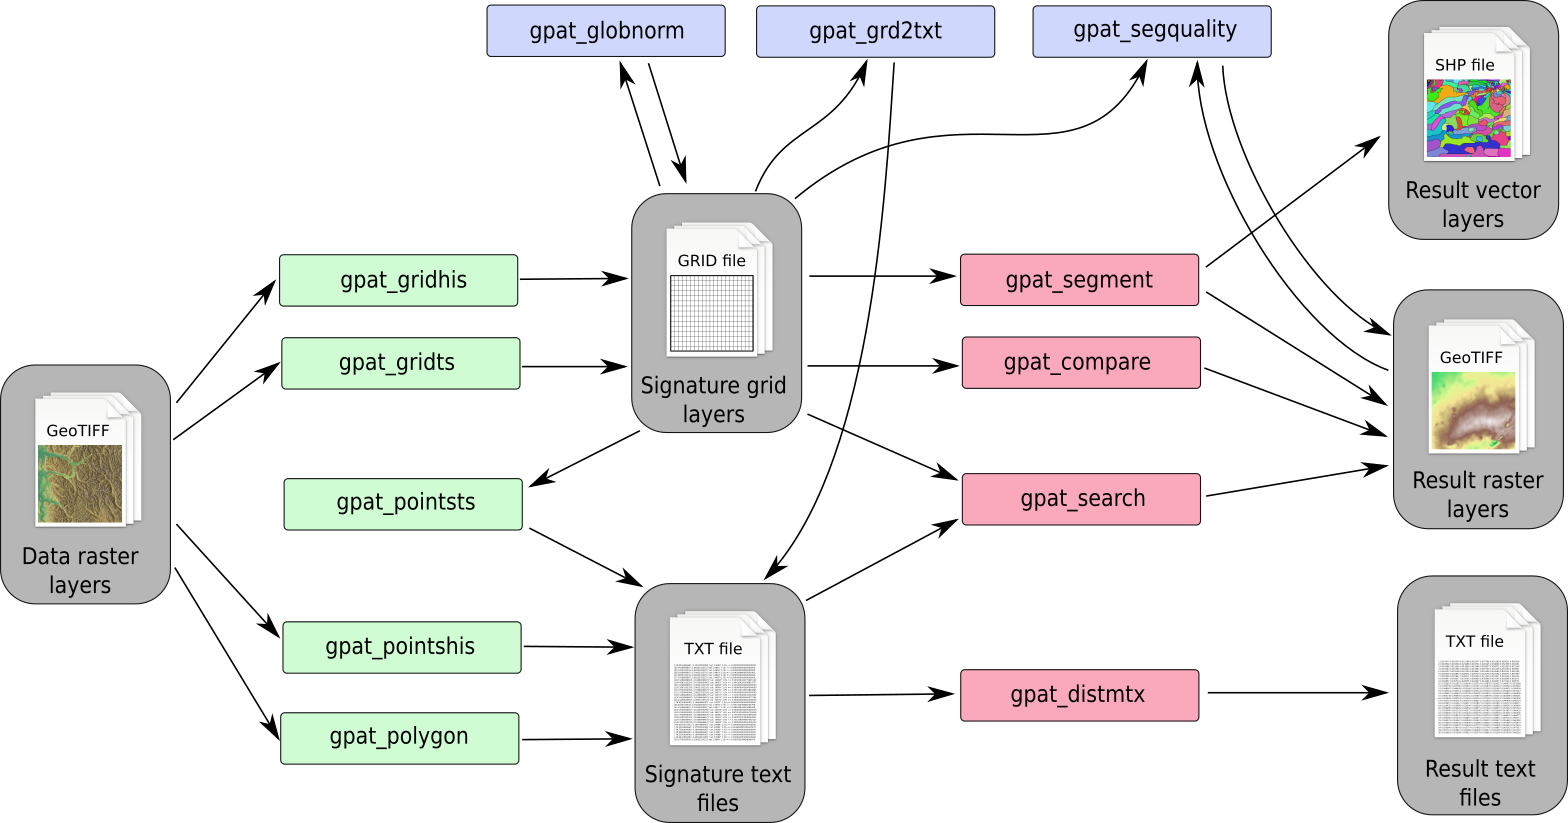
\includegraphics[width=1.1\textwidth]{GPAT2.png}}
	\caption{Outline of GeoPAT 2.0 architecture.}
	\label{FIG:GPAT} 
\end{figure}

\subsection{GeoPAT Modules}

\subsubsection{Signature building}

\newparagraph{gpat\_gridhis}
Creates a binary grid of signatures from a categorical raster map(s).
\\\\
Usage:

\begin{minipage}{\linewidth}
\begin{lstlisting}
gpat_gridhis [-lh] -i <file_name> -o <file_name> [-s <signature_name>] [--level=<n>] [-z <n>] [-f <n>] [-n <normalization_name>] [-t <n>]

-i, --input=<file_name>    name of input file (GeoTIFF)
-o, --output=<file_name>   name of output file (GRID)
-s, --signature=<name>     motifel's signature (use -l to list all signatures, default: 'cooc')
--level=<n>                full decomposition level (default: 0, auto)
-z, --size=<n>             motifel size in cells (default: 150)
-f, --shift=<n>            shift of motifels (default: 100)
-n, --normalization=<name> signature normalization method (use -l to list all methods, default: 'pdf')
-l                         list all signatures and normalization methods
-t <n>                     number of threads (default: 1)
-h, --help                 print this help and exit
\end{lstlisting}
\end{minipage}

{\bf Options:}

\newoption{input}

Defines a categorical raster layer(s) which will be used as a source for extracting pattern signature.
Layers must be a categorical one. For the Cartesian product method ('prod') there can be more than one input map.
Other methods use a one map only (the first one provided). 
In order to provide more than one input map, type multiple input options ("-i map1.tif -i map2.tif" or "--input=map1.tif --input=map2.tif").

\newoption{output}

Output consists of two files: one of them is a dataset containing a grid of signatures in binary form, the other one is a header text file (the .hdr extension) containing a grid topology and an information about the input data parameters.
Modifying the header is strongly discouraged as tt may cause some calculations to fail. 
Structure of the header is as follows:\\

\begin{itemize}
	\item dim -- number of dimensions of each signature
	\item dims -- size of each dimension
	\item type -- type of data stored in the grid (integer, float, etc.)
	\item at0 -- top left x
	\item at1 -- w-e grid resolution
	\item at2 -- rotation (0 if grid is north-up)
	\item at3 -- top left y
	\item at4 -- rotation (0 if grid is north-up)
	\item at5 -- n-s grid resolution
	\item rows -- number of rows in the grid
	\item cols -- number of cols in the grid
	\item proj -- projection in wkt style
	\item desc -- command used to create the grid
\end{itemize}

\newoption{size}

Size of a motifel (local calculation window) expressed in the number of pixels. 
It defines the extent of a local pattern.
It is the length of the side of square-shaped block of pixels (motifel).
It must be at least 10 and cannot exceed the input map size.

\newoption{shift}

Parameter defines the shift between adjacent scenes along the grid in n-s and w-e directions. 
It describes the density of the output gird and defines a new topology of the grid.
Formula original\_resolution $\times$ shift = new\_resolution explains how resolution of the original map will be reduced. 
If shift is set to the same value as 'size', the input map will be simply divided into a grid of non-overlapping motifels. 
Setting shift to a value smaller than 'size' parameter will result in grid of overlapping motifels. 
Shift cannot be larger than 'size', and cannot be smaller than 5.

\newoption{signature}

Defines method of calculating signatures of motifels. GeoPAT offers the following methods: 
\begin{itemize}
	\item prod -- Cartesian product of input category lists
	\item cooc -- spatial coocurrence of categories
	\item sdec -- simple 2-level decomposition
	\item fdec -- full decomposition
	\item lbp -- histogram of local binary patterns
	\item lind -- landscape indices vector
	\item linds -- selected landscape indices vector
\end{itemize}
See Appendix \ref{signatures} for the details.

\newoption{level}

This option is used only if 'full decomposition' (fdec) is used.
It defines the highest level of decomposition. See Appendix \ref{signatures} for the details.

\newoption{normalization}

Specifies normalization method used on the signatures. 
See Appendix \ref{signatures} for the details.

\newoption{threads (-t)}

The module is parallel, therefore use more than one processing thread can be used in order to speed up calculations. 
This option specifies how many threads will be used. 
The default is 1.
\\\\

{\bf Description:}

This module extracts a "grid-of-scenes" (grid of pattern signatures, grid of motifels).
The output is a grid of the same spatial extent as the input raster map, but with a different cell size.
Each cell in a new grid has only one attribute - the signature of its pattern. 
Pattern is calculated over a window centered on the cell and having a user-defined size.
Resolution of the output grid equals to the resolution of the input raster map multiplied by the shift parameter. 
A signature of pattern for each scene is stored as a numerical vector in a binary form.
The module outputs a header file (.hdr) containing a topology of a grid-of-scenes and a binary file containing signatures ordered by rows.

This module uses categorical raster data in GeoTIFF format as an input. 
It might be more than one map for the Cartesian product signature. 
Raster maps must be categorical and its size must be greater than the scene size specified by the user. 
Size defines the size of individual scene for which the histogram is calculated. 
Shift shows how scenes shift along the grid in n-s and w-e directions. 
Shift defines the resolution of the new grid.
If window size is bigger than shift (recommended), motifels will overlap.
If shift and size is equal, windows will not overlap. Shift cannot be greater than size. 

The output grid may be an input to one of the following GeoPAT modules: {\it gpat\_search, gpat\_compare, gpat\_segment, gpat\_segquality, gpat\_grd2txt, and gpat\_globnorm}.

\newparagraph{gpat\_gridts}
{}
\\\\
Usage:

\begin{minipage}{\linewidth}
\begin{lstlisting}
gpat_gridts [-nh] -i <file_name> [-i <file_name>]... -o <file_name> [-d <n>]

-i, --input=<file_name>  name of input file(s) (GeoTIFF)
-o, --output=<file_name> name of output file (GRID)
-d, --dimension=<n>      dimension of vector that describes time series element (default: 1)
-n, --normalize          normalize each vector coordinate to [0.0, 1.0] (default: no)
-h, --help               print this help and exit
\end{lstlisting}
\end{minipage}

\newoption{input}

\newoption{output}

\newoption{dimension}

\newoption{normalize}

% \\\\
{\bf Description:}

\newparagraph{gpat\_pointshis}
Calculates numerical signatures of individual motifels within a raster map.
\\\\
Usage:

\begin{minipage}{\linewidth}
\begin{lstlisting}
gpat_pointshis [-lah] -i <file_name> -o <file_name> [-s <signature_name>] [--level=<n>] [-z <n>] [-n <normalization_name>] [-x <double>] [-y <double>] [-d <string>] [--xy_file=<file_name>]

-i, --input=<file_name>    name of input file (GeoTIFF)
-o, --output=<file_name>   name of output file (TXT)
-s, --signature=<name>     motifel's signature (use -l to list all signatures, default: 'cooc')
--level=<n>                full decomposition level (default: 0, auto)
-z, --size=<n>             motifel size in cells (default: 150)
-n, --normalization=<name> signature normalization method (use -l to list all methods, default: 'pdf')
-l                         list all signatures and normalization methods
-x <double>                x coord
-y <double>                y coord
-d, --description=<string> description of the location
--xy_file=<file_name>      name of file with coordinates (TXT)
-a, --append               append results to output file
-h, --help                 print this help and exit
\end{lstlisting}
\end{minipage}

{\bf Options:}

\newoption{input}

Defines categorical raster map(s) in the GeoTIFF format, which will be used as a source for extracting pattern signature.
For the Cartesian product method ('prod') there can be more than one input map. 
Other methods use one map only (the first one provided). 
In order to provide more than one input map, type multiple input options ("-i map1.tif -i map2.tif" or "--input=map1.tif --input=map2.tif").

\newoption{output}

Name of output text file containing signatures. 
In the output file, each line corresponds to a single motifel's signature. 
Each signature is preceded by its header.
A header always consists of: coordinates of the midpoint of motifel (scene), name, number of dimensions, and length of each dimension. 
Modifying the signature file is strongly discouraged as it may cause some calculations to fail.

\newoption{signature}

Defines method for calculating signatures of motifels.
GeoPAT offers the following methods: 
\begin{itemize}
	\item prod -- Cartesian product of input category lists
	\item cooc -- spatial coocurrence of categories
	\item sdec -- simple 2-level decomposition
	\item fdec -- full decomposition
	\item lbp -- histogram of local binary patterns
	\item lind -- landscape indices vector
	\item linds -- selected landscape indices vector
\end{itemize}
See Appendix \ref{signatures} for details.

\newoption{level}

This option is used only when 'full decomposition' (fdec) is used.
It defines the highest level of decomposition.
See Appendix \ref{signatures} for the details.

\newoption{size}

Size of a motifel (scene) for which signature is calculated.
Scene is a square centered at the coordinate pair location, while its extent is defined by size. 

\newoption{normalization}

Specifies normalization method used on the signatures. 
See Appendix \ref{signatures} for the details.

\newoption{x}

X coordinate of the midpoint of motifel for which signature will be calculated.

\newoption{y}

Y coordinate of the midpoint of motifel for which signature will be calculated.

\newoption{description}

Description of a motifel.
It can be a name of location, description of pattern, or anything else. 
If not provided, the default description is "location".

\newoption{xy\_file}

Name of a text file with list of coordinates. 
This option is useful for calculating signatures for multiple motifels in a single run. 

\newoption{append} (flag)

Append mode. 
Useful when using the coordinate pair mode and when scenes are processed one by one (see description below). 
If the append flag is used and the output file already exists, signatures will be appended at the end of file instead of overwriting it.
\\\\
{\bf Description:}

This module extracts signatures for a scene (motifel) or collection of scenes defined over square-shaped windows.
User provides coordinates of the center of each scene and the size of the scene. 
The module outputs a list of scene-labeled signatures.
As an input the module uses categorical raster map in the GeoTIFF format (or a few maps if user calculates the Cartesian product of multiple maps), coordinates of the center of each scene and size of scenes. 
The coordinates must be in the input map's coordinate system. 
There are two ways of defining the scenes:

Definition by coordinate pair: 
This is the simplest mode designed for a batch or interactive processing. 
In this mode, scene is defined by a pair of its midpoint's coordinates (the {\it x} and {\it y} options) and scene size parameter (the {\it size} option). 
Only one scene can be processed at once. 
The {\it xy\_file} option is not used in this mode.
If used with the append flag (-a), signatures can be calculated one by one and added to the same output file. 
Additionally, the {\it description} option lets user name a scene. 
This name will be stored in the output file.

Definition by text file:
In this mode, scene midpoint's coordinates are defined in a external text file in which each line contains X,Y coordinates and, optionally, name/description using the following syntax: x\_coordinate,y\_coordinate,scene\_name.
The name of a file with coordinates is provided using the {\it xy\_file} option. 
Extent of a scene is defined by the {\it size} parameter. 
The {\it x, y} and {\it description} options are not used in this mode. 
Example of the content of coordinates file: 

\begin{minipage}{\linewidth}
\begin{lstlisting}
1289255,1271313,forest
1306271,1272740,city
1268560,1264726
\end{lstlisting}
\end{minipage}

If a description is not provided (like in the example above), the program will assign a default name ("location") with id representing the number of line in the coordinate file.

The output signature text file can be used as an input to the following modules: {\it gpat\_search}, {\it gpat\_distmtx}.

\newparagraph{gpat\_pointsts}
{}
\\\\
Usage:

\begin{minipage}{\linewidth}
\begin{lstlisting}
gpat_pointsts [-ah] -i <file_name> -o <file_name> [-x <double>] [-y <double>] [-d <string>] [--xy_file=<file_name>]

-i, --input=<file_name>    name of input file (GRID)
-o, --output=<file_name>   name of output file (TXT)
-x <double>                x coord
-y <double>                y coord
-d, --description=<string> description of the location
--xy_file=<file_name>      name of file with coordinates (TXT)
-a, --append               append results to output file
-h, --help                 print this help and exit
\end{lstlisting}
\end{minipage}

\newoption{input}

\newoption{output}

\newoption{x coord (-x)}

\newoption{y coord (-y)}

\newoption{description}

\newoption{xy\_file}

\newoption{append}

% \\\\
{\bf Description:}

\newparagraph{gpat\_polygon}
Calculates numerical signatures of irregular regions.
\\\\
Usage:

\begin{minipage}{\linewidth}
\begin{lstlisting}
gpat_polygon [-lh] -i <file_name> -e <file_name> -o <file_name> [-s <signature_name>] [-n <normalization_name>] [-t <n>]

-i, --input=<file_name>    name of input file (GeoTIFF)
-e, --segments=<file_name> name of input file (GeoTIFF, int)
-o, --output=<file_name>   name of output file (TXT)
-s, --signature=<name>     signature method (use -l to list all methods, default: 'cooc')
-n, --normalization=<name> signature normalization method (use -l to list all methods, default: 'pdf')
-l                         list all signatures and normalization methods
-t <n>                     number of threads (default: 1)
-h, --help                 print this help and exit
\end{lstlisting}
\end{minipage}

{\bf Options:}

\newoption{input}

Categorical raster map(s) in the GeoTIFF format, which will be used as a source for extracting pattern signature. 
For the Cartesian product method ('prod') there can be more than one input map. 
Other methods only use one map (the first one provided). 
In order to provide more than one input map, type multiple input options ("-i map1.tif -i map2.tif" or "--input=map1.tif --input=map2.tif").

\newoption{segments}

Categorical raster map in the GeoTIFF format which defines spatial division of area of interest into polygonal regions.
In this map, regions should be defined as areas of unique ids. 
Layer must be a raster and its projection, extents and resolution should be identical to the main input map. 
This layer may be a result of the segmentation module {\it gpat\_segment} or any other categorical map (e.g. map of ids of watersheds).

\newoption{output}

Name of output text file containing signatures. 
In the output file each line corresponds to a region's signature.
Each signature is preceded by its header. 
A header always consists of: the coordinates of the midpoint of region, name, number of dimensions, and length of each dimension. 
Modifying the signature file is strongly discouraged as it may cause some calculations to fail.

\newoption{signature}

Defines method for calculating signatures of motifels. 
GeoPAT offers the following methods: 
\begin{itemize}
	\item prod -- Cartesian product of input category lists
	\item cooc -- spatial coocurrence of categories
	\item sdec -- simple 2-level decomposition
	\item fdec -- full decomposition
	\item lbp -- histogram of local binary patterns
	\item lind -- landscape indices vector
	\item linds -- selected landscape indices vector
\end{itemize}
See Appendix \ref{signatures} for the details.

\newoption{normalization}

Specifies normalization method used on the signatures. 
See Appendix \ref{signatures} for the details.

\newoption{threads (-t)}

The module is parallel, therefore use more than one processing thread can be used in order to speed up calculations. 
This option specifies how many threads will be used. 
The default is 1.
\\\\
{\bf Description:}

Module extracts signatures for a collection of irregular regions using the same methods as in the {\it gpat\_pointshis} and {\it gpat\_gridhis} modules. 
As an input, apart from categorical raster map from which signatures are calculated, user provides a categorical raster map which defines spatial division of area of interest into polygonal regions. 
The module outputs a list of polygon labeled-signatures stored in the form of a text file. 
Output can be transferred to the p.sim.distmatrix for further processing.

The output signature text file can be used as an input to the following modules: {\it gpat\_search}, {\it gpat\_distmtx}.

\subsubsection{Similarity measuring}

\newparagraph{gpat\_search}
Produces similarity maps which show similarity value between query motifels (scenes) and every motifel in the input grid.
\\\\
Usage:

\begin{minipage}{\linewidth}
\begin{lstlisting}
gpat_search [-dlh] -i <file_name> [-o <file_name>] -r <file_name> [-m <measure_name>] [--type=Byte/....] [-p <file_name>] [-n <n>] [-t <n>]

-i, --input=<file_name>      name of input file (GRID)
-o, --output=<file_name>     name of output file (TIFF)
-r, --reference=<file_name>  reference data to calculate similarity (TXT)
-d, --description            use description of the reference histogram(s) as name of output file(s)
-m, --measure=<measure_name> similarity measure (use -l to list all measures; default 'jsd')
-l, --list_measures          list all measures
--type=Byte/....             output data type (default: Float64)
-p, --palette=<file_name>    name of the file with colors definition (CSV)
-n, --no_data=<n>            output NO DATA value (default: none)
-t <n>                       number of threads (default: 1)
-h, --help                   print this help and exit
\end{lstlisting}
\end{minipage}

\newoption{input}

Binary file containing grid of signatures (grid-of-scenes). 
Grid is mandatory. 
User has to provide a name of grid file (without the .hdr extension). 
Header file is read automatically. 
Grid is an output from either {\it gpat\_gridhis} or {\it gpat\_gridts} module. 
Header of the grid will define topology of the output layers. 
Do not modify header file.

\newoption{output}

\newoption{reference}

Text file containing one or more signatures of either individual motifels (scenes) or irregular polygons. 
This option is mandatory. 
Input text file can be created using the {\it gpat\_pointshis}, {\it gpat\_pointsts} or {\it gpat\_polygons} module. 
The number of outputs depends on the number of scenes in the input scene file. 
At least one scene is required. 
%??Name/description of  will be used to create name of output layer. 

\newoption{description}

\newoption{measure}

\newoption{list\_measures}

\newoption{type}

\newoption{palette}

\newoption{no\_data}

\newoption{threads (-t)}

% \\\\
{\bf Description:}

\newparagraph{gpat\_compare}
{}
\\\\
Usage:

\begin{minipage}{\linewidth}
\begin{lstlisting}
gpat_compare [-lh] -i <file_name> -i <file_name> -o <file_name> [--type=Byte/....] [-p <file_name>] [-n <n>] [-m <measure_name>] [-t <n>]

-i, --input=<file_name>      name of input files (GRID)
-o, --output=<file_name>     name of output file with similarity (TIFF)
--type=Byte/....             output data type (default: Float64)
-p, --palette=<file_name>    name of the file with colors definition (CSV)
-n, --no_data=<n>            output NO DATA value (default: none)
-m, --measure=<measure_name> similarity measure (use -l to list all measures; default 'jsd')
-l, --list_measures          list all measures
-t <n>                       number of threads (default: 1)
-h, --help                   print this help and exit
\end{lstlisting}
\end{minipage}

\newoption{input}

\newoption{output}

\newoption{type}

\newoption{palette}

\newoption{no\_data}

\newoption{measure}

\newoption{list\_measures}

\newoption{threads (-t)}

% \\\\
{\bf Description:}

\newparagraph{gpat\_segment}
{}
\\\\
Usage:

\begin{minipage}{\linewidth}
\begin{lstlisting}
gpat_segment [-lcgaqh] -i <file_name> -o <file_name> [-v <file_name>] [--size=<n>] [-m <measure_name>] [--lthreshold=<double>] [--uthreshold=<double>] [--swap=<double>] [--minarea=<n>] [--maxhist=<n>] [-t <n>]

-i, --input=<file_name>  name of input files (GRID)
-o, --output=<file_name> name of output file with segments (TIFF)
-v, --vector=<file_name> name of output vector file with segments (SHP)
--size=<n>               output resolution modyfier (default: 1)
-m, --measure=<name>     similarity measure (use -l to list all measures; defult: jsd)
-l, --list_measures      list all measures
--lthreshold=<double>    minimum distance threshold to build areas (default: 0.1)
--uthreshold=<double>    maximum distance threshold to build areas (default: 0.3)
--swap=<double>          improve segmentation by swapping unmatched areas. -1 to skip (default: 0.001)
--minarea=<n>            minimum number of motifels in individual segment (default: 0)
--maxhist=<n>            create similarity/distance matrix for maxhist histograms; leave 0 to use all (default: 200)
-c, --complete           use complete linkage (default is average)
-g, --no_growing         skip growing phase
-a, --no_hierarhical     skip herarhical phase
-q, --quad               quad mode (rook topology)
-t <n>                   number of threads (default: 1)
-h, --help               print help and exit
\end{lstlisting}
\end{minipage}

\newoption{input}

\newoption{output}

\newoption{vector}

\newoption{size}

\newoption{measure}

\newoption{list\_measures}

\newoption{lthreshold}

\newoption{uthreshold}

\newoption{swap}

\newoption{minarea}

\newoption{maxhist}

\newoption{complete}

\newoption{no\_growing}

\newoption{no\_hierarhical}

\newoption{quad}

\newoption{threads (-t)}

% \\\\
{\bf Description:}

\newparagraph{gpat\_distmtx}
{}
\\\\
Usage:

\begin{minipage}{\linewidth}
\begin{lstlisting}
gpat_distmtx [-lsh] -i <file_name> -o <file_name> [-m <measure_name>]

-i, --input=<file_name>  name of input file witch signatures (TXT)
-o, --output=<file_name> name of output file (CSV) with similarity matrix
-m, --measure=<name>     similarity measure (use -l to list all measures; default 'jsd')
-l, --list_measures      list all measures
-s, --similarity         output is a similarity matrix
-h, --help               print this help and exit
\end{lstlisting}
\end{minipage}

\newoption{input}

\newoption{output}

\newoption{measure}

\newoption{list\_measures}

\newoption{similarity}

% \\\\
{\bf Description:}

\subsubsection{Tools}
\newparagraph{gpat\_grd2txt}
{}
\\\\
Usage:

\begin{minipage}{\linewidth}
\begin{lstlisting}
gpat_grd2txt [-h] -i <file_name> -o <file_name>

-i, --input=<file_name>   name of input file (GRID)
-o, --output=<file_name>  name of output file (TXT)
-h, --help                print this help and exit
\end{lstlisting}
\end{minipage}

\newoption{input}

\newoption{output}

% \\\\
{\bf Description:}

\newparagraph{gpat\_globnorm}
{}
\\\\
Usage:

\begin{minipage}{\linewidth}
\begin{lstlisting}
gpat_globnorm [-lh] -i <file_name> -o <file_name> [-m <method_name>] [-t <n>]

-i, --input=<file_name>   name of input file (GRID)
-o, --output=<file_name>  name of output file (GRID)
-m, --method=<method_name> normalization method (use -l to list all methods, default: '01')
-l, --list_methods        list all methods
-t <n>                    number of threads (default: 1)
-h, --help                print this help and exit
\end{lstlisting}
\end{minipage}

\newoption{input}

\newoption{output}

\newoption{method}

\newoption{list\_methods}

\newoption{threads (-t)}

% \\\\
{\bf Description:}

\newparagraph{gpat\_segquality}
{}
\\\\
Usage:

\begin{minipage}{\linewidth}
\begin{lstlisting}
gpat_segquality [-lcqwh] -i <file_name> -s <file name> [-g <file_name>] [-o <file_name>] [-m <measure_name>] [--maxhist=<n>] [-t <n>]

-i, --input=<file_name>     name of input file (GRID)
-s, --segments=<file name>  name of input segmentation map (TIFF)
-g, --inhomogeneity=<file_name> name of output file with segment inhomogeneity (TIF
F)
-o, --isolation=<file_name> name of output file with segment isolation (TIFF)
-m, --measure=<name>        similarity measure (use -l to list all measures; defult: jsd)
-l, --list_measures         list all measures
--maxhist=<n>               create similarity/distance matrix for maxhist histograms; leave 0 to use all (default: 200)
-c, --complete            use complete linkage (default is average)
-q, --quad                quad mode (rook topology)
-w, --no_weight           switch off edge-based weighting in isolation
-t <n>                    number of threads (default: 1)
-h, --help                print help and exit
\end{lstlisting}
\end{minipage}

\newoption{input}

\newoption{segments}

\newoption{inhomogeneity}

\newoption{isolation}

\newoption{measure}

\newoption{list\_measures}

\newoption{maxhist}

\newoption{complete}

\newoption{quad}

\newoption{no\_weight}

\newoption{threads (-t)}

% \\\\
{\bf Description:}